\documentclass[a4paper, 11pt]{article}
\usepackage{comment} % enables the use of multi-line comments (\ifx \fi) 
\usepackage{fullpage} % changes the margin

\usepackage{tabu} % for nice arrays	
% For confusion matrix %
\usepackage{array}
\usepackage{multirow}

\newcommand\MyBox[2]{
  \fbox{\lower0.75cm
     \vbox to 1.7cm{\vfil
      \hbox to 1.7cm{\hfil\parbox{1.4cm}{#1\\#2}\hfil}
      \vfil}%
   }%
}
%%%%%%%%%%%%%%%%%%%%%%%%%
\usepackage{graphicx} % For img insert
\newcommand{\ts}{\textsuperscript} %For numering 1st 2nd
%% Greek Format %%
%\usepackage[cm-default]{fontspec}
%\setromanfont{FreeSerif}
%\setsansfont{FreeSans}
%\setmonofont{FreeMono}
\usepackage{xltxtra}
\usepackage{xgreek}
\setmainfont[Mapping=tex-text]{GFS Didot}
%%%%%%%%%%%%%%%%%%

\begin{document}
%Header-Make sure you update this information!!!!
\noindent
\large\textbf{Ανάλυση FPR} \hfill \textbf{Αθανάσιος Μητσέλος} \\
\normalsize ΣΗΜΜΥ \hfill Ημερομηνία Ανάθεσης: 06/12/16  \\
ΕΜΠ\hfill Τρέχουσα Ημερομηνία: 09/05/17 \\


\section*{Εισαγωγή}
Στην παρούσα αναφορά θα γίνει παρουσίαση και ανάλυση των καταναλωτών που εκλαμβάνονται από τον αλγόριθμο μερικώς επιβλεπόμενης μάθησης σαν ύποπτα δείγματα, ενώ στην πραγματικότητα οι μετρήσεις τους είναι άθικτες. Με την ανάλυση αυτών των συμπεριφορών καθίσταται ευκολότερος ο επανασχεδιασμός του αλγορίθμου για να μην ενοχοποιεί τέτοιου είδους καταναλωτές. Όπως γίνεται σαφές η ελαχιστοποίηση των λαθών είναι καίριας σημασίας ειδικά όταν το λάθος ενοχοποιεί κάποιο καταναλωτή. \\
Σε κάθε καταναλωτή έχουν εκχωρηθεί κάποια χαρακτηριστικά που δεν θα αναλυθούν σε αυτή την αναφορά. Τα χαρακτηριστικά είναι τα εξής:    
\begin{enumerate}
\item{\textit{Ετήσια μέση τιμή ημίωρου}} Βρίσκεται ο μέσος όρος ημίωρου κάθε μέρας και για όλες τις μέρες του έτους βρίσκεται ο ετήσιος μέσος όρος.
\item{\textit{Ετήσια τυπική απόκλιση ημίωρου}} Βρίσκεται η τυπική απόκλιση κάθε μέρας και για όλες τις μέρες του έτους βρίσκεται ο ετήσιος μέσος όρος της τυπικής απόκλισης.
\item{\textit{Κινούμενος μέσος όρος μηνιαίου μέσου όρου}} Πρόκειται για υπό συνθήκη χαρακτηριστικό που αν παρατηρήσει κάποια σημαντική πτώση των καταναλώσεων τότε ψάχνει για την μέγιστη και την καταγράφει. 
\item{\textit{Κινούμενος μέσος όρος μηνιαίας τυπικής απόκλισης}} Πρόκειται για υπό συνθήκη χαρακτηριστικό που αν παρατηρήσει κάποια σημαντική πτώση της τυπικής απόκλισης τότε ψάχνει για την μέγιστη και την καταγράφει.
\item{\textit{Συμμετρική διαφορά καταναλώσεων}} Πρόκειται για υπό συνθήκη χαρακτηριστικό που παρατηρεί μια γενική συμπεριφορά όμοιων καταναλωτών ως προς τη χρονική στιγμή της ελάχιστης κατανάλωσης και ψάχνει για κάποια σημαντική πτώση της κατανάλωσης ανάμεσα σε 2 συμμετρικές χρονικές στιγμές με άξονα συμμετρίας την εκάστοτε χρονική στιγμή ελαχίστου.
\item{\textit{Συμμετρική διαφορά τυπικής απόκλισης}} Πρόκειται για υπό συνθήκη χαρακτηριστικό που παρατηρεί μια γενική συμπεριφορά όμοιων καταναλωτών ως προς τη χρονική στιγμή της ελάχιστης κατανάλωσης και ψάχνει για κάποια σημαντική πτώση της τυπικής απόκλισης ανάμεσα σε 2 συμμετρικές χρονικές στιγμές με άξονα συμμετρίας την εκάστοτε χρονική στιγμή ελαχίστου.
\item{\textit{Τμηματική διαφορά κατανάλωσης με όμοιους καταναλωτές}} Πρόκειται για υπό συνθήκη χαρακτηριστικό που παρατηρεί μια γενική συμπεριφορά όμοιων καταναλωτών ως προς τη χρονική στιγμή της ελάχιστης κατανάλωσης και ψάχνει για κάποια σημαντική πτώση της κατανάλωσης ανάμεσα στον καταναλωτή και τους όμοιούς του μετά την χρονική στιγμή της ελάχιστης κατανάλωσης.
\item{\textit{Τμηματική διαφορά τυπικής απόκλισης με όμοιους καταναλωτές}} Πρόκειται για υπό συνθήκη χαρακτηριστικό που παρατηρεί μια γενική συμπεριφορά όμοιων καταναλωτών ως προς τη χρονική στιγμή της ελάχιστης κατανάλωσης και ψάχνει για κάποια σημαντική πτώση της τυπικής απόκλισης ανάμεσα στον καταναλωτή και τους όμοιούς του μετά την χρονική στιγμή της ελάχιστης κατανάλωσης.
\end{enumerate}

\section*{Παράδειγμα 1}
\begin{figure}[ht!]
\centering
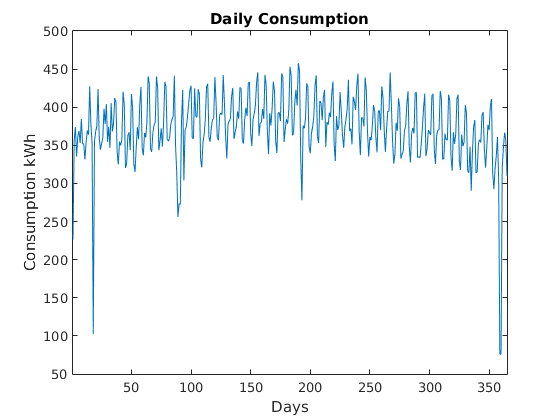
\includegraphics[width=100mm, height=70mm]{../../plots/FPR_analysis/Example_1.png}
\caption{Παράδειγμα 1\label{exFPR1}}
\end{figure}

\begin{center}
\begin{tabu} to 0.8\textwidth { | X[c] | X[c] | X[c] | X[c] | X[c] | X[c] | X[c] | X[c] |  }
 \hline
 \multicolumn{8}{|c|}{Χαρακτηριστικά 1ου Παραδείγματος} \\
 \hline
 1 & 2 & 3  & 4 & 5 & 6 & 7 & 8 \\
 \hline
15.55 &  14.48   &      0      &   0    &     0    &    0 & 132.5 & 0\\
\hline
\end{tabu}
\end{center}


\section*{Παράδειγμα 2}
\begin{figure}[ht!]
\centering
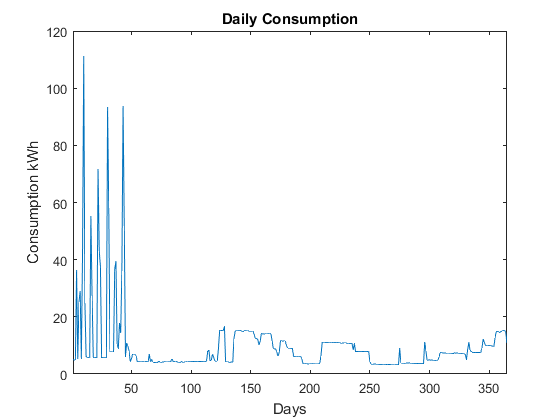
\includegraphics[width=100mm, height=70mm]{../../plots/FPR_analysis/Example_2.png}
\caption{Παράδειγμα 2\label{exFPR2}}
\end{figure}

\begin{center}
\begin{tabu} to 0.8\textwidth { | X[c] | X[c] | X[c] | X[c] | X[c] | X[c] | X[c] | X[c] |  }
 \hline
 \multicolumn{8}{|c|}{Χαρακτηριστικά 2ου Παραδείγματος} \\
 \hline
 1 & 2 & 3  & 4 & 5 & 6 & 7 & 8 \\
 \hline
0.4  &  0.17 &    0 & 0.64  & 1.84 &  1.84 &  8.058 &   0.56\\
\hline
\end{tabu}
\end{center}

\section*{Παράδειγμα 3}
\begin{figure}[ht!]
\centering
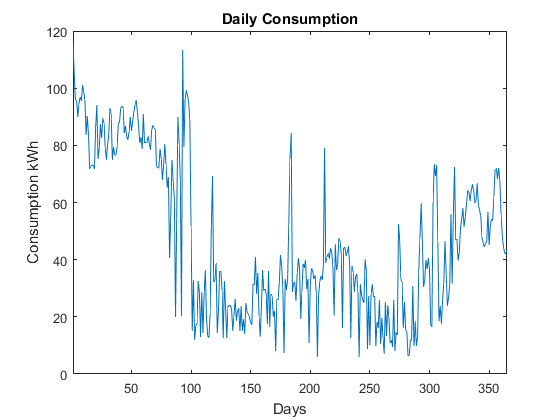
\includegraphics[width=100mm, height=70mm]{../../plots/FPR_analysis/Example_3.png}
\caption{Παράδειγμα 3\label{exFPR3}}
\end{figure}

\begin{center}
\begin{tabu} to 0.8\textwidth { | X[c] | X[c] | X[c] | X[c] | X[c] | X[c] | X[c] | X[c] |  }
 \hline
 \multicolumn{8}{|c|}{Χαρακτηριστικά 3ου Παραδείγματος} \\
 \hline
 1 & 2 & 3  & 4 & 5 & 6 & 7 & 8 \\
 \hline
1.95  &  0.98   &     0   &     0  & 16.79   &     0   &      0  &  0.3\\
\hline
\end{tabu}
\end{center}

\section*{Παράδειγμα 4}
\begin{figure}[ht!]
\centering
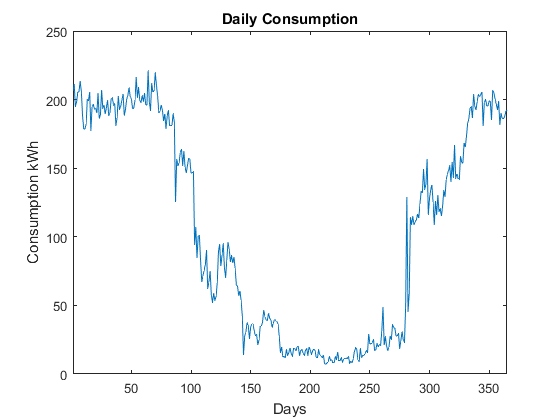
\includegraphics[width=100mm, height=70mm]{../../plots/FPR_analysis/Example_4.png}
\caption{Παράδειγμα 4\label{exFPR4}}
\end{figure}

\begin{center}
\begin{tabu} to 0.8\textwidth { | X[c] | X[c] | X[c] | X[c] | X[c] | X[c] | X[c] | X[c] |  }
 \hline
 \multicolumn{8}{|c|}{Χαρακτηριστικά 4ου Παραδείγματος} \\
 \hline
 1 & 2 & 3  & 4 & 5 & 6 & 7 & 8 \\
 \hline
4.42   & 5.37  & 0  &  0  & 20.82 &  20.82  & 10.09   &      0\\
\hline
\end{tabu}
\end{center}

\section*{Παράδειγμα 5}
\begin{figure}[ht!]
\centering
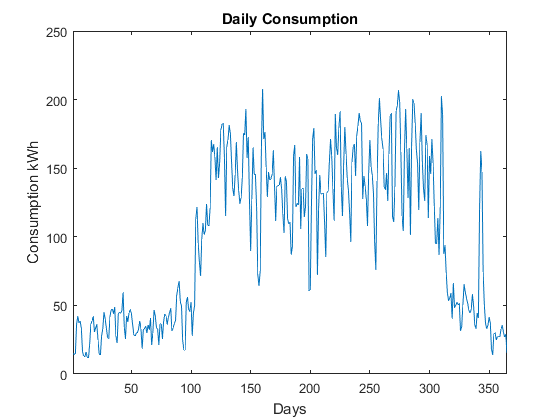
\includegraphics[width=100mm, height=70mm]{../../plots/FPR_analysis/Example_5.png}
\caption{Παράδειγμα 5\label{exFPR5}}
\end{figure}

\begin{center}
\begin{tabu} to 0.8\textwidth { | X[c] | X[c] | X[c] | X[c] | X[c] | X[c] | X[c] | X[c] |  }
 \hline
 \multicolumn{8}{|c|}{Χαρακτηριστικά 5ου Παραδείγματος} \\
 \hline
 1 & 2 & 3  & 4 & 5 & 6 & 7 & 8 \\
 \hline
4.11  &  1.66   &    0   &      0    &     0 &        0    &     0  &  0.85\\
\hline
\end{tabu}
\end{center}

\section*{Παράδειγμα 6}
\begin{figure}[ht!]
\centering
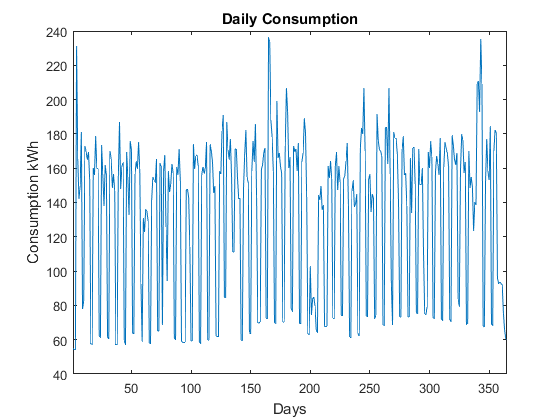
\includegraphics[width=100mm, height=70mm]{../../plots/FPR_analysis/Example_6.png}
\caption{Παράδειγμα 5\label{exFPR6}}
\end{figure}

\begin{center}
\begin{tabu} to 0.8\textwidth { | X[c] | X[c] | X[c] | X[c] | X[c] | X[c] | X[c] | X[c] |  }
 \hline
 \multicolumn{8}{|c|}{Χαρακτηριστικά 6ου Παραδείγματος} \\
 \hline
 1 & 2 & 3  & 4 & 5 & 6 & 7 & 8 \\
 \hline
5.52   & 3.15 &        0     &    0      &   0   & 1.72  &       0   &      0\\
\hline
\end{tabu}
\end{center}

\section*{Παράδειγμα 7}
\begin{figure}[ht!]
\centering
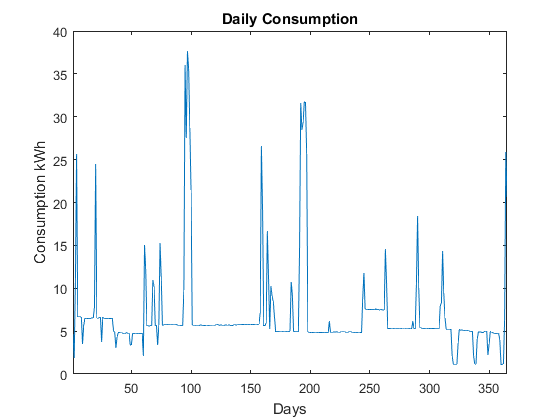
\includegraphics[width=100mm, height=70mm]{../../plots/FPR_analysis/Example_7.png}
\caption{Παράδειγμα 5\label{exFPR7}}
\end{figure}

\begin{center}
\begin{tabu} to 0.8\textwidth { | X[c] | X[c] | X[c] | X[c] | X[c] | X[c] | X[c] | X[c] |  }
 \hline
 \multicolumn{8}{|c|}{Χαρακτηριστικά 7ου Παραδείγματος} \\
 \hline
 1 & 2 & 3  & 4 & 5 & 6 & 7 & 8 \\
 \hline
0.29 &   0.14    &     0    &     0   & 2.28  &  2.28  &  9.66  &  0.54\\
\hline
\end{tabu}
\end{center}

\section*{Παρατηρήσεις}
Παραπάνω φαίνονται 7 γενικευμένες συμπεριφορές που ο αλγόριθμος ενοχοποιεί χωρίς ωστόσο ο καταναλωτής να έχει αλλοιώσει τα δεδομένα του. Σε όλα τα παραδείγματα, οι χρονοσειρές αποκλίνουν σημαντικά από τις χρονοσείρες των υπόλοιπων ομοίων. Ειδικότερα:
\begin{itemize}
\item Οι χρονοσειρές \ref{exFPR1} και \ref{exFPR6} φαίνονται να έχουν μεγάλη εποχιακότητα και επαναληψιμότητα χωρίς ωστόσο να φαίνεται πως μπορούν να γενικευτούν από μια παραβολική κυματομορφή, όπως οι υπόλοιποι. Αντιθέτως, η γενίκευση της κυματομορφής μπορεί να γίνει από μια ευθεία με πολύ μικρή κλίση, δηλαδή δεν έχει στατιστικό ενδιαφέρον η τετραγωνική τάση. Ουσιαστικά πρόκειται για επιχειρήσεις που έχουν έντονες, συνεχείς, αλλά προβλέψιμες διακυμάνσεις χωρίς όμως να αλλάζουν τις καταναλωτικές τους συνήθειες ανά εποχή του έτους. 
\item Οι χρονοσειρές \ref{exFPR2} και \ref{exFPR7} παρόλο που και αυτές δεν μπορούν να γενικευτούν με μια τετραγωνική συνάρτηση ή τάση δείχνουν έντονη έλλειψη εποχιακότητας. Ειδικότερα, παρουσιάζουν τελείως τυχαίες διακυμάνσεις και σταθερές καταναλώσεις για μεγάλα χρονικά διαστήματα. Κάτι τέτοιο υποδεικνύει πως οικιακό καταναλωτή που λείπει από την κατοικία του για τυχαία και μεγάλα χρονικά διαστήματα, αφήνοντας κάποιες ή και καμιά συσκευή να λειτουργεί.
\item Οι χρονοσειρές \ref{exFPR3} και \ref{exFPR4} ακολουθούν εποχιακή επαναληψιμότητα και μπορούν να γενικευτούν με μια παραβολική καμπύλη. Παρόλα αυτά, το ελάχιστο της χρονοσειράς έχει σημαντική μετακίνηση προς τα δεξιά και έντονη κλίση στην αλλαγή των εποχών του έτους, δημιουργώντας βίαιες μεταβολές στα χαρακτηριστικά που σχετίζονται με τους μέσους όρους. Πρόκειται για μικρές επιχειρήσεις που επηρεάζονται σημαντικά από την εποχή του έτους, αλλά οι ενεργειακές τους απαιτήσεις δεν βασίζονται σε αυτή τη μεταβλητή.
\item Η χρονοσειρά \ref{exFPR5} παρουσιάζει εποχιακότητα και μπορεί να γενικευτεί από μια αρνητική παραβολική συνάρτηση. Το συγκεκριμένο παράδειγμα είναι παρουσιάζει την ακριβώς αντίστροφη συμπεριφορά από αυτήν που αναμενόταν έχοντας το κύριο μέρος της κατανάλωσής της στο σημείου που οι υπόλοιποι έχουν το ελάχιστο. Αυτό υποδεικνύει μια επιχείρηση με έντονο φόρτο εργασίας το διάστημα που οι υπόλοιποι καταναλωτές έχουν χαμηλές καταναλώσεις.
\end{itemize}



\section*{Συνημμένα}
\ifx
Lab Notes, HelloWorld.ic, FooBar.ic,
\ref{exFPR1}.
\fi %comment me out
\ref{exFPR1}. Παράδειγμα 1, \ref{exFPR2}. Παράδειγμα 2, \ref{exFPR3}. Παράδειγμα 3, \ref{exFPR4}. Παράδειγμα 4, \ref{exFPR5}. Παράδειγμα 5, \ref{exFPR6}. Παράδειγμα 6, \ref{exFPR7}. Παράδειγμα 7


\end{document}
